\documentclass[letter]{article}

\usepackage{enumitem}
\usepackage{listings}
\usepackage{color}
\usepackage{float}
\usepackage{graphicx}
\usepackage{amsmath}

\graphicspath{ {./Figures/} }

\definecolor{dkgreen}{rgb}{0,0.6,0}
\definecolor{gray}{rgb}{0.5,0.5,0.5}
\definecolor{mauve}{rgb}{0.58,0,0.82}

\lstset{frame=tb,
  language=Python,
  aboveskip=3mm,
  belowskip=3mm,
  showstringspaces=false,
  columns=flexible,
  basicstyle={\small\ttfamily},
  numbers=none,
  numberstyle=\tiny\color{gray},
  keywordstyle=\color{blue},
  commentstyle=\color{dkgreen},
  stringstyle=\color{mauve},
  breaklines=true,
  breakatwhitespace=true,
  tabsize=3
}

\begin{document}

\section{Neural Networks using Numpy}

\subsection{Helper Functions}

\subsubsection{Activation Function}

\textit{The function \texttt{np.maximum()} performs an element-wise maximum comparison, which provides is more efficient and simplistic than the other comparison functions such as \texttt{np.max()} and \texttt{np.amax()}.}

\begin{lstlisting}
def relu(x):
    return np.maximum(0, x)
\end{lstlisting}

$\textbf{ReLU}(x) = \max(x, 0)$ \\

\subsubsection{Softmax Function}

\textit{To avoid overflows while computing exponentials, the maximum of the input array is subtracted from each value before performing the softmax.}

\begin{lstlisting}
def softmax(x):
    x = x - np.max(x, axis=1, keepdims=True)
    return np.exp(x) / np.sum(np.exp(x), axis=1, keepdims=True)
\end{lstlisting}

$\sigma(z)_j = \frac{e^{z_j}}{\sum_{k = 1}^K e^{z_k}}$ \\

\subsubsection{Compute Prediction}

\textit{The inputs comes first in the matrix multiplication due to the way in which the inputs values are formatted in the matrix: the row vectors represent the input values of one training sample.}

\begin{lstlisting}
def compute_layer(x, w, b):
    return np.matmul(x, w) + b
\end{lstlisting}

$z = Wx + b$ \\

\subsubsection{Average Cross-Entropy Loss}

\begin{lstlisting}
def average_ce(target, prediction):
    return -np.mean(np.sum((target * np.log(prediction)), axis=1))
\end{lstlisting}

$\textbf{CE}_{avg} = -\frac{1}{N} \sum_{n = 1}^N \sum_{k = 1}^K y_k^{(n)} \log\left(p_k^{(n)}\right)$ \\

\subsubsection{Gradient of Average Cross-Entropy Loss}

\textit{It is important that that gradient computed is of the average cross-entropy loss, and not the normal cross-entropy loss. Although this will not result in major changes, the gradient will be the average of gradient of the cross-entropy loss.} \\

\noindent
To make the derivation simpler, we will let the output of the softmax for the $k$\textsuperscript{th} class $\sigma(z)_k$ be represented by $p_k$, the input of the softmax $\textbf{o}$ be represented by $z$, and the average cross-entropy loss function $\textbf{CE}_{avg}$ be represented by simply $L$. Furthermore, the derivative can be broken down into constituent parts as such.

\begin{align} \label{eqn:1}
\frac{\partial{L}}{\partial{z}} = \frac{\partial{L}}{\partial{p}} \frac{\partial{p}}{\partial{z}}
\end{align}

\noindent
To calculate the full gradient, we must consider all class outputs of the softmax function derived with respect to the logits of every class. The gradient below requires the quotient derivative rule.

\begin{align*}
\frac{\partial{p_i}}{\partial{z_j}} &= \frac{\partial{}}{\partial{z_j}} \frac{e^{z_i}}{\sum_{k = 1}^K e^{z_k}} \\
&=
\begin{cases}
    \frac{e^{z_i} \left(\sum_{k = 1}^K e^{z_k}\right) - e^{z_j} e^{z_i}}{\left(\sum_{k = 1}^K e^{z_k}\right)^2} & \text{if } i = j \\
    \frac{0 - e^{z_j} e^{z_i}}{\left(\sum_{k = 1}^K e^{z_k}\right)^2} & \text{otherwise}
\end{cases} \\
&=
\begin{cases}
    \frac{e^{z_i} \left[ \left(\sum_{k = 1}^K e^{z_k}\right) - e^{z_j} \right]}{\left(\sum_{k = 1}^K e^{z_k}\right)^2} & \\
    \frac{-e^{z_j} e^{z_i}}{\left(\sum_{k = 1}^K e^{z_k}\right)^2} &
\end{cases} \\
&=
\begin{cases}
    \frac{e^{z_i}}{\left(\sum_{k = 1}^K e^{z_k}\right)} \frac{\left(\sum_{k = 1}^K e^{z_k}\right) - e^{z_j}}{\left(\sum_{k = 1}^K e^{z_k}\right)} & \\
    \frac{-e^{z_j}}{\left(\sum_{k = 1}^K e^{z_k}\right)} \frac{e^{z_i}}{\left(\sum_{k = 1}^K e^{z_k}\right)} &
\end{cases} \\
&= \label{eqn:2} \tag{2}
\begin{cases}
    p_i (1 - p_j) & \\
    -p_j p_i &
\end{cases}
\end{align*}

\newpage

\noindent
Now we can derive the gradient of the average cross-entropy by substituting the derivation we got above equation \ref{eqn:2} into the full gradient through the chain rule we derived from equation \ref{eqn:1}.

\begin{align*}
\frac{\partial{L}}{\partial{z}} &= \frac{\partial{L}}{\partial{p}} \frac{\partial{p}}{\partial{z}} \\
&= \frac{\partial{}}{\partial{p}} \left[ -\frac{1}{N} \sum_{n = 1}^N \sum_{k = 1}^K y_k^{(n)} \log\left(p_k^{(n)}\right) \right] \frac{\partial{p}}{\partial{z}} \\
&= -\frac{1}{N} \sum_{n = 1}^N \sum_{k = 1}^K y_k^{(n)} \frac{1}{p_k^{(n)}} \frac{\partial{p}}{\partial{z}} \\
&= -\frac{1}{N} \sum_{n = 1}^N \left[ y_i^{(n)} \frac{1}{p_i^{(n)}} \left( p_i^{(n)} (1 - p_i^{(n)}) \right) + \sum_{k \neq i} y_k^{(n)} \frac{1}{p_k^{(n)}} \left( -p_k^{(n)} p_i^{(n)} \right) \right] \\
&= -\frac{1}{N} \sum_{n = 1}^N \left[ y_i^{(n)} (1 - p_i^{(n)}) - \sum_{k \neq i} y_k^{(n)} p_i^{(n)} \right] \\
&= -\frac{1}{N} \sum_{n = 1}^N \left[ y_i^{(n)} - y_i^{(n)} p_i^{(n)} - \sum_{k \neq i} y_k^{(n)} p_i^{(n)} \right] \\
&= -\frac{1}{N} \sum_{n = 1}^N \left[ y_i^{(n)} - p_i^{(n)} \left( y_i^{(n)} + \sum_{k \neq i} y_k^{(n)} \right) \right] \\
&= -\frac{1}{N} \sum_{n = 1}^N \left[ y_i^{(n)} - p_i^{(n)} \sum_{k = 1}^K y_k^{(n)} \right] \\
&= \frac{1}{N} \sum_{n = 1}^N \left( p_i^{(n)} - y_i^{(n)} \right) \label{eqn:3} \tag{3}
\end{align*}

\noindent
As we can see from equation \ref{eqn:3}, the gradient comes to a lovely reduction to the average of the differences between logits of the predictions and the true labels. 

\begin{lstlisting}
def grad_ce(target, logits):
    return np.mean(softmax(logits) - target, axis=0, keepdims=True)
\end{lstlisting}

\newpage

\subsection{Backpropagation Derivation} \label{backprop}

Since we are taking the gradient with respect to the weights at the output and hidden layer, we will need to incorporate the activations from the input layer $\textbf{a}_i$, hidden layer $\textbf{a}_h$, and output layer $\textbf{a}_o$. The respective values for each unit $i$ is denoted as $a_i^{(i)}$, $a_i^{(h)}$, and $a_i^{(o)}$. For simplicity, the total cross-entropy loss is used both in calculating the gradients and in the \texttt{Numpy} implementation.

\subsubsection{Output Layer Weights}

\begin{align*}
\frac{\partial{L}}{\partial{\textbf{W}_o}} &= \frac{\partial{L}}{\partial{\textbf{z}_o}} \frac{\partial{\textbf{z}_o}}{\partial{\textbf{W}_o}} \\
&= \left( \textbf{a}_o - \textbf{y} \right) \frac{\partial{}}{\partial{\textbf{W}_o}} \left[ \textbf{W}_o \textbf{a}_h + \textbf{b}_o \right] \\
&= \textbf{a}_h^T \left( \textbf{a}_o - \textbf{y} \right)
\end{align*}

\subsubsection{Output Layer Biases}

\begin{align*}
\frac{\partial{L}}{\partial{\textbf{b}_o}} &= \frac{\partial{L}}{\partial{\textbf{z}_o}} \frac{\partial{\textbf{z}_o}}{\partial{\textbf{b}_o}} \\
&= \left( \textbf{a}_o - \textbf{y} \right) \frac{\partial{}}{\partial{\textbf{b}_o}} \left[ \textbf{W}_o \textbf{a}_h + \textbf{b}_o \right] \\
&= \textbf{1}^T \left( \textbf{a}_o - \textbf{y} \right)
\end{align*}

\subsubsection{Hidden Layer Weights}

\begin{align*}
\frac{\partial{L}}{\partial{\textbf{W}_h}} &= \frac{\partial{L}}{\partial{\textbf{z}_o}} \frac{\partial{\textbf{z}_o}}{\partial{\textbf{a}_h}} \frac{\partial{\textbf{a}_h}}{\partial{\textbf{z}_h}}
\frac{\partial{\textbf{z}_h}}{\partial{\textbf{W}_h}} \\
&= 
\begin{cases}
	\left( a_i^{(o)} - y_i \right) \left(W_i^{(o)}\right)^T \left(a_i^{(i)}\right) & \text{if } z_i^{(h)} > 0 \\
	0 & \text{otherwise}
\end{cases}
\end{align*}

\subsubsection{Hidden Layer Biases}

\begin{align*}
\frac{\partial{L}}{\partial{\textbf{W}_h}} &= \frac{\partial{L}}{\partial{\textbf{z}_o}} \frac{\partial{\textbf{z}_o}}{\partial{\textbf{a}_h}} \frac{\partial{\textbf{a}_h}}{\partial{\textbf{z}_h}}
\frac{\partial{\textbf{z}_h}}{\partial{\textbf{b}_h}} \\
&= 
\begin{cases}
	\left( a_i^{(o)} - y_i \right) \left(W_i^{(o)}\right)^T & \text{if } z_i^{(h)} > 0 \\
	0 & \text{otherwise}
\end{cases}
\end{align*}

\newpage

\subsection{Learning}

\begin{figure}[H]
	\centering
	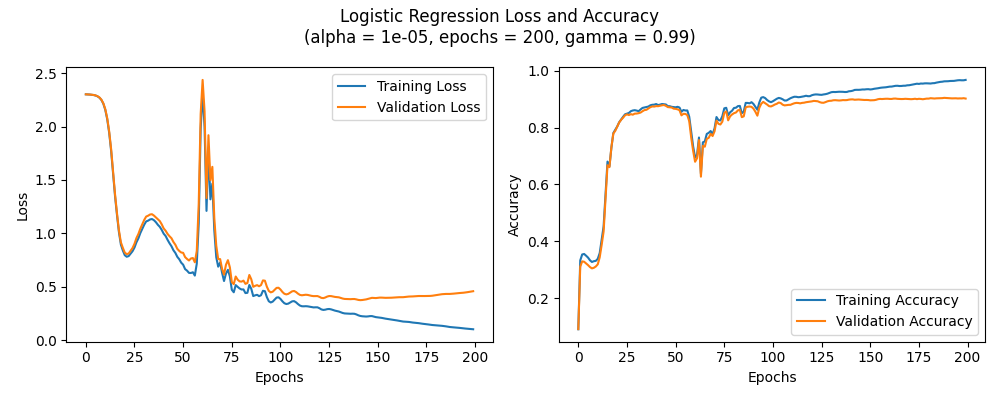
\includegraphics[width=\linewidth]{Figure_1}
	\label{fig:plot1}
\end{figure}

As mentioned in section \ref{backprop}, the \texttt{Numpy} model was trained using total cross-entropy loss and its gradients for simplicity. The learning rate was scaled down to $\alpha = 10^{-5}$ to adjust for the difference. Despite the large instability spikes between epoch $50$ and epoch $75$, the network stabilizes afterwards for a final training accuracy of $96.8\%$, validation accuracy of $90.2\%$, and testing accuracy of $90.1\%$. 

\end{document}
